% --- I-JEPA Overview ---
\begin{frame}{I-JEPA: Image Joint Embedding Predictive Architecture}
  \begin{itemize}
    \item Introduced by Meta AI (Assran et al., 2023) as an instantiation of Yann LeCun's \textbf{Joint Embedding Predictive Architecture} vision: learn an \emph{internal model} of the world by comparing \textbf{abstract representations} rather than raw pixels.
    \item Self-supervised from unlabeled images; targets are \textbf{feature embeddings} of masked regions predicted from visible context, not pixel reconstruction.
  \end{itemize}
\end{frame}

% --- I-JEPA: Why Predict Features, Not Pixels? ---
\begin{frame}{I-JEPA: Why Predict Features, Not Pixels?}
  \begin{itemize}
    \item Generative objectives often try to explain \textbf{every} missing detail even when the world is \textbf{stochastic} at pixel level---wasting capacity on irrelevant variation (Meta blog example: hands in generative models).
    \item Predicting \textbf{embeddings} steers the model toward \textbf{stable, high-level} structure: objects, parts, and layout.
    \item Empirically: strong \textbf{linear probing} and \textbf{semi-supervised} transfer; competitive on some \textbf{low-level} tasks (e.g.\ counting, depth) despite simpler augmentation than many contrastive methods.
  \end{itemize}
\end{frame}

% --- I-JEPA: Model Architecture ---
\begin{frame}{I-JEPA: Model Architecture (Meta)}
  \begin{columns}[T,onlytextwidth]
    \column{0.5\textwidth}
  \centering
      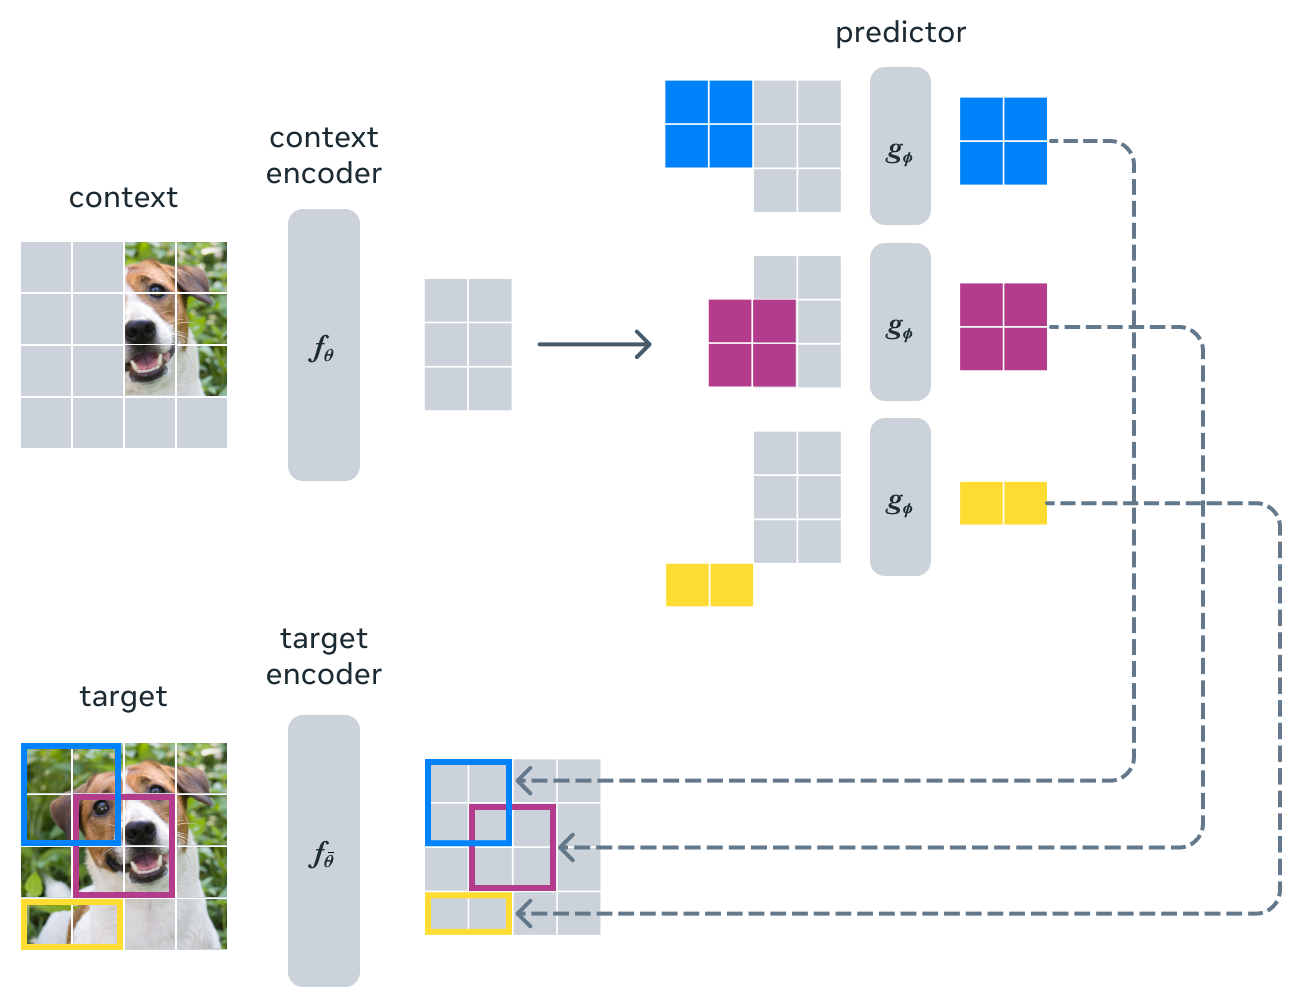
\includegraphics[width=0.95\textwidth, height=0.95\textheight, keepaspectratio]{assets/New-Lecture_JEPA_models/ijepa_blog_architecture.png}
      {\scriptsize Reference: Meta I-JEPA blog architecture.}
    \column{0.5\textwidth}
  \begin{itemize}
        \item \textbf{Context encoder} ($f_\theta$): ViT on \textbf{visible} patches only.
        \item \textbf{Predictor} ($g_\phi$): narrow ViT that maps context tokens + target \textbf{positional} information to predicted embeddings for each target block.
        \item \textbf{Target encoder} ($f_{\bar{\theta}}$): encodes full image for targets; weights track the context encoder via \textbf{exponential moving average} (EMA), not gradient through targets.
        \item Training minimizes distance between predicted and target \textbf{embeddings}.
  \end{itemize}
  \end{columns}
\end{frame}


% --- I-JEPA: Key Principles ---
% \begin{frame}{I-JEPA: Key Principles and Multi-Block Masking}
%   \begin{itemize}
%     \item SSL objective lives in \textbf{embedding space}: the model predicts \textbf{representations} of target blocks, not pixels.
%     \item One or more large \textbf{context} regions provide an informative, spatially distributed view; \textbf{target} blocks are separate regions whose embeddings must be predicted---\textbf{multi-block masking} at a scale that carries \textbf{semantic} content (not tiny random patches).
%     \item The predictor is a \textbf{restricted world model} for \textbf{static} images: it reasons about what is plausible in unseen regions given partial observation.
%     \item Loss: match predicted target embeddings to those from the \textbf{target encoder} (with stop-gradient / EMA updates---see architecture slide).
%   \end{itemize}
% \end{frame}


% --- I-JEPA: Training Dynamics ---
% \begin{frame}{I-JEPA: Training and Implementation}
%   \begin{itemize}
%     \item Sample multi-block masks; for each target block, predict its embedding from context tokens and target position encodings.
%     \item \textbf{No multi-view contrastive pipeline:} unlike many SSL methods, I-JEPA avoids expensive pipelines that process many augmented views per step---only context blocks need the context encoder pass; target path uses a single view for targets.
%     \item Feature-space loss (e.g.\ MSE) + EMA target network for stable targets; avoids collapse without pixel reconstruction.
%     \item Mask design (large semantic targets, informative context) is a core inductive bias---more important than hand-crafted view augmentations for this family.
%   \end{itemize}
% \end{frame}

% --- I-JEPA: Semantic visualization (Meta blog) ---
\begin{frame}{I-JEPA: What Do Predicted Embeddings Encode?}
  \begin{columns}[T,onlytextwidth]
    \column{0.42\textwidth}
    \begin{itemize}\itemsep0.35em
      \item To \textbf{visualize} what the predictor represents, Meta trains a \textbf{stochastic decoder} that maps predicted embeddings toward \textbf{pixel sketches} inside a blue box (for analysis only---not the training objective).
      \item The model tends to capture \textbf{object parts} and \textbf{pose} (e.g.\ dog's head, wolf legs, building structure) rather than arbitrary texture noise.
  \end{itemize}
    \column{0.56\textwidth}
    \centering
    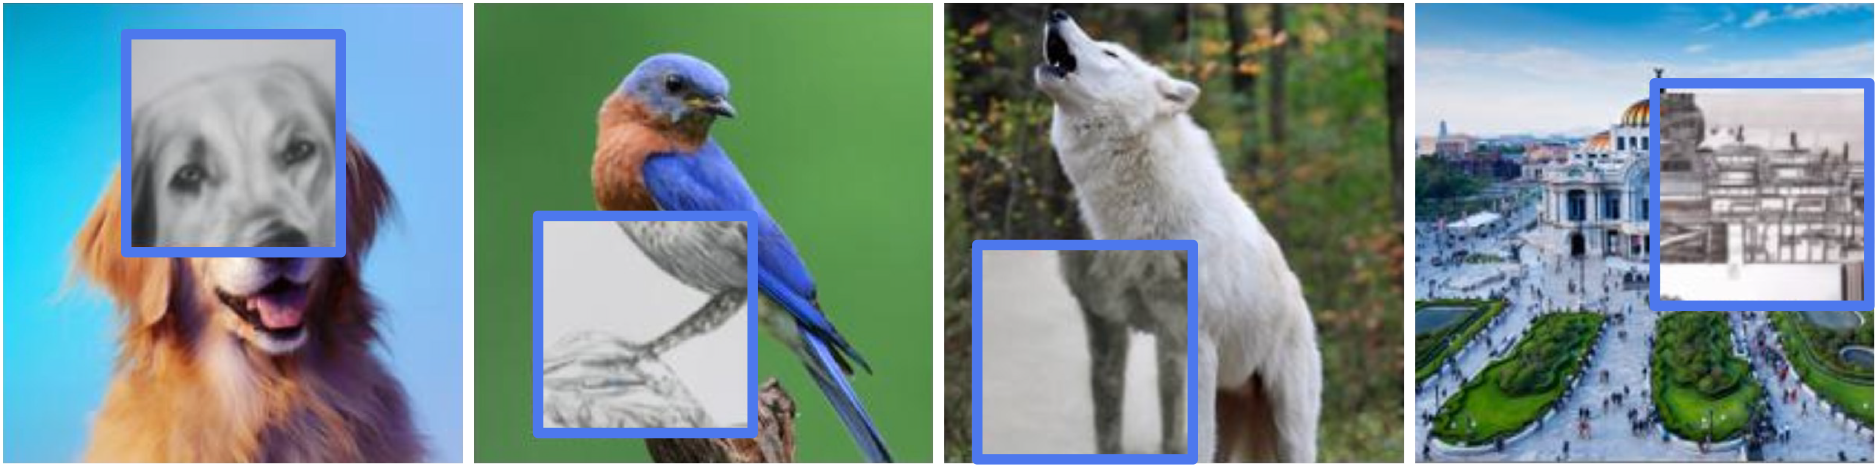
\includegraphics[width=0.95\textwidth, height=0.95\textheight, keepaspectratio]{assets/New-Lecture_JEPA_models/ijepa_blog_semantic_sketches.png}\\[0.2em]
    {\scriptsize Illustrating how the predictor learns to model the semantics of the world. For each image, the portion outside of the blue box is encoded and given to the predictor as context. The predictor outputs a representation for what it expects to be in the region within the blue box. To visualize the prediction, we train a generative model that produces a sketch of the contents represented by the predictor output, and we show a sample output within the blue box. Clearly the predictor recognizes the semantics of what parts should be filled in (the top of the dog's head, the bird's leg, the wolf's legs, the other side of the building).
    }
  \end{columns}
\end{frame}

% --- I-JEPA: Compute efficiency (Meta blog) ---
% \begin{frame}{I-JEPA: Evaluation}
%   \begin{columns}[T,onlytextwidth]
%     \column{0.38\textwidth}
%     \begin{itemize}\itemsep0.3em
%       \item On ImageNet-1K \textbf{linear evaluation}, I-JEPA reaches strong accuracy at fewer \textbf{pretraining GPU-hours} than several masking and reconstruction baselines (e.g.\ MAE, data2vec) in Meta's reported comparison.
%       \item Intuition: representation prediction avoids heavy per-pixel decoder compute and focuses learning on features that transfer.
%     \end{itemize}
%     \column{0.6\textwidth}
%     \centering
%     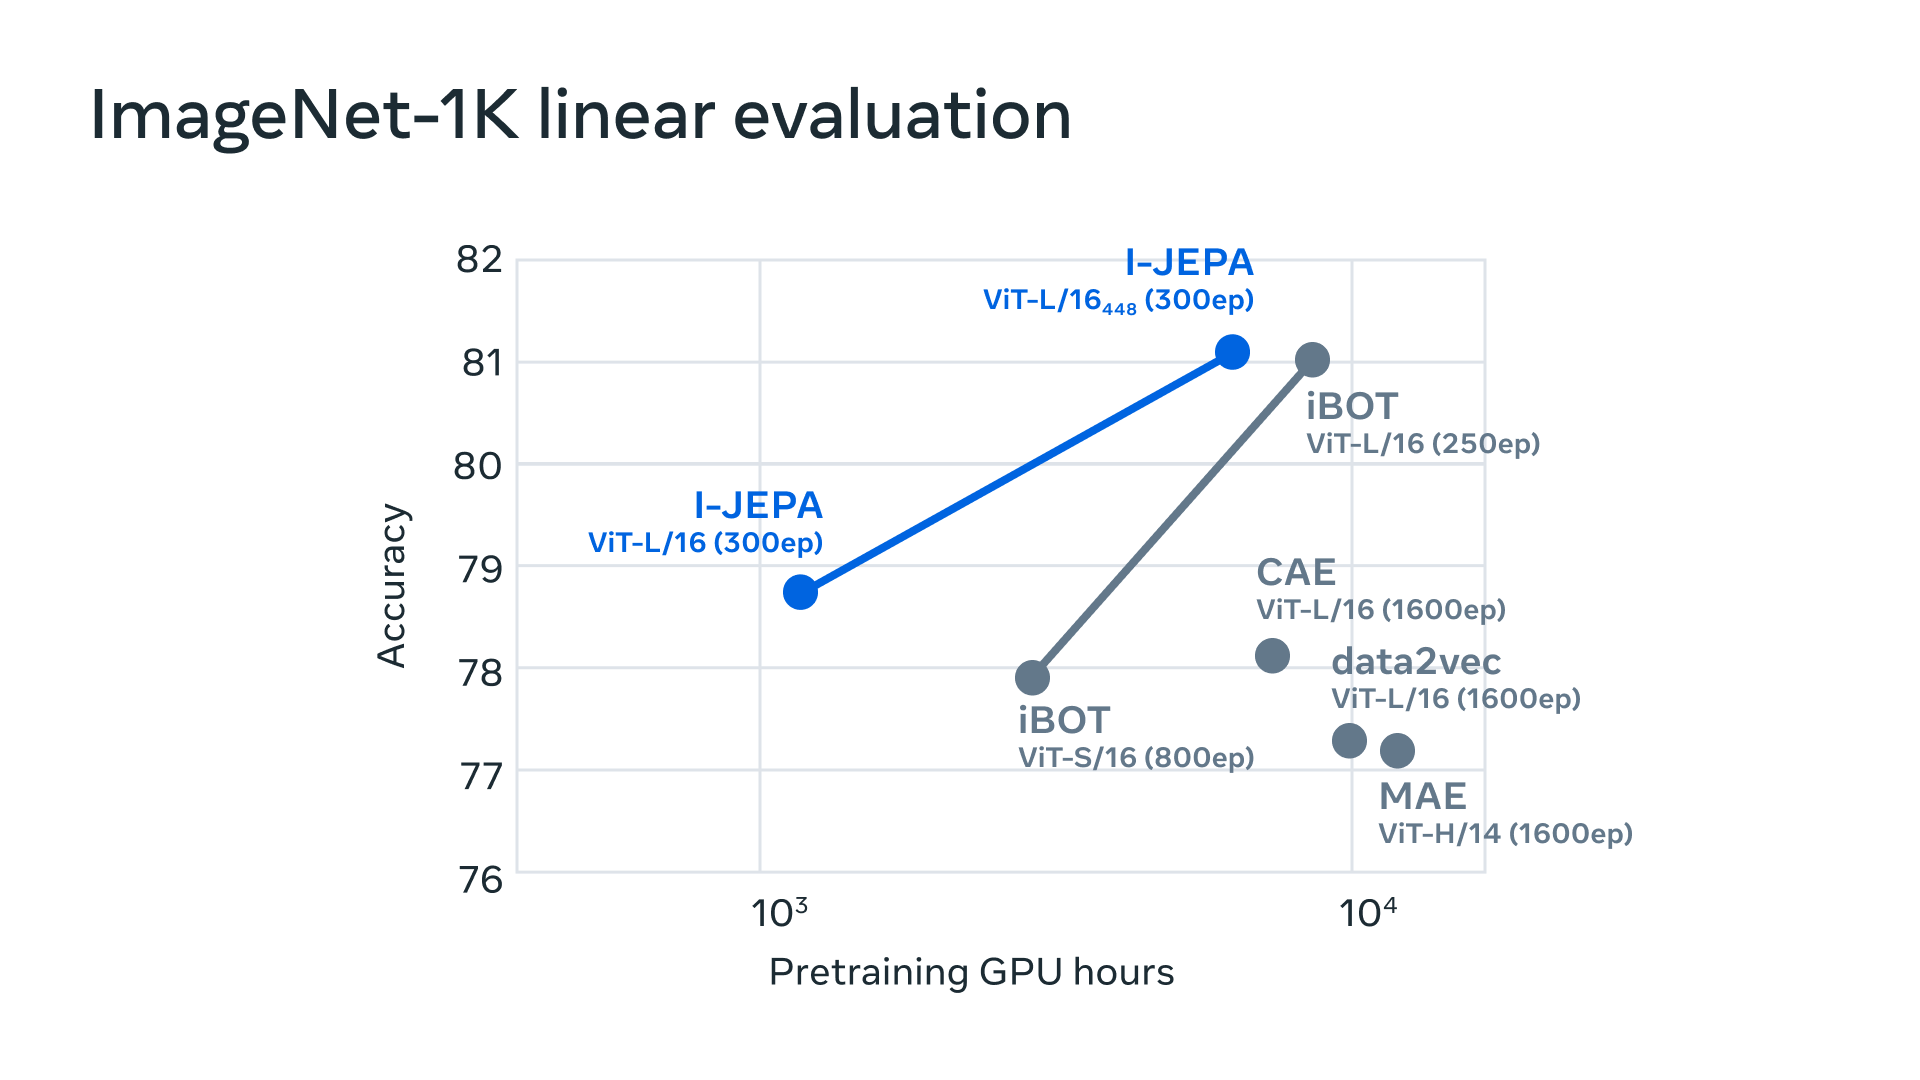
\includegraphics[width=0.8\linewidth, height=0.8\textheight, keepaspectratio]{assets/New-Lecture_JEPA_models/ijepa_blog_gpu_hours_linear_eval.png}\\[0.2em]
%     {\scriptsize ImageNet-1K linear eval vs.\ GPU hours (Meta).}
%   \end{columns}
% \end{frame}

% --- I-JEPA: ImageNet table (Meta blog) ---
\begin{frame}{I-JEPA: Evaluation}
  \centering
  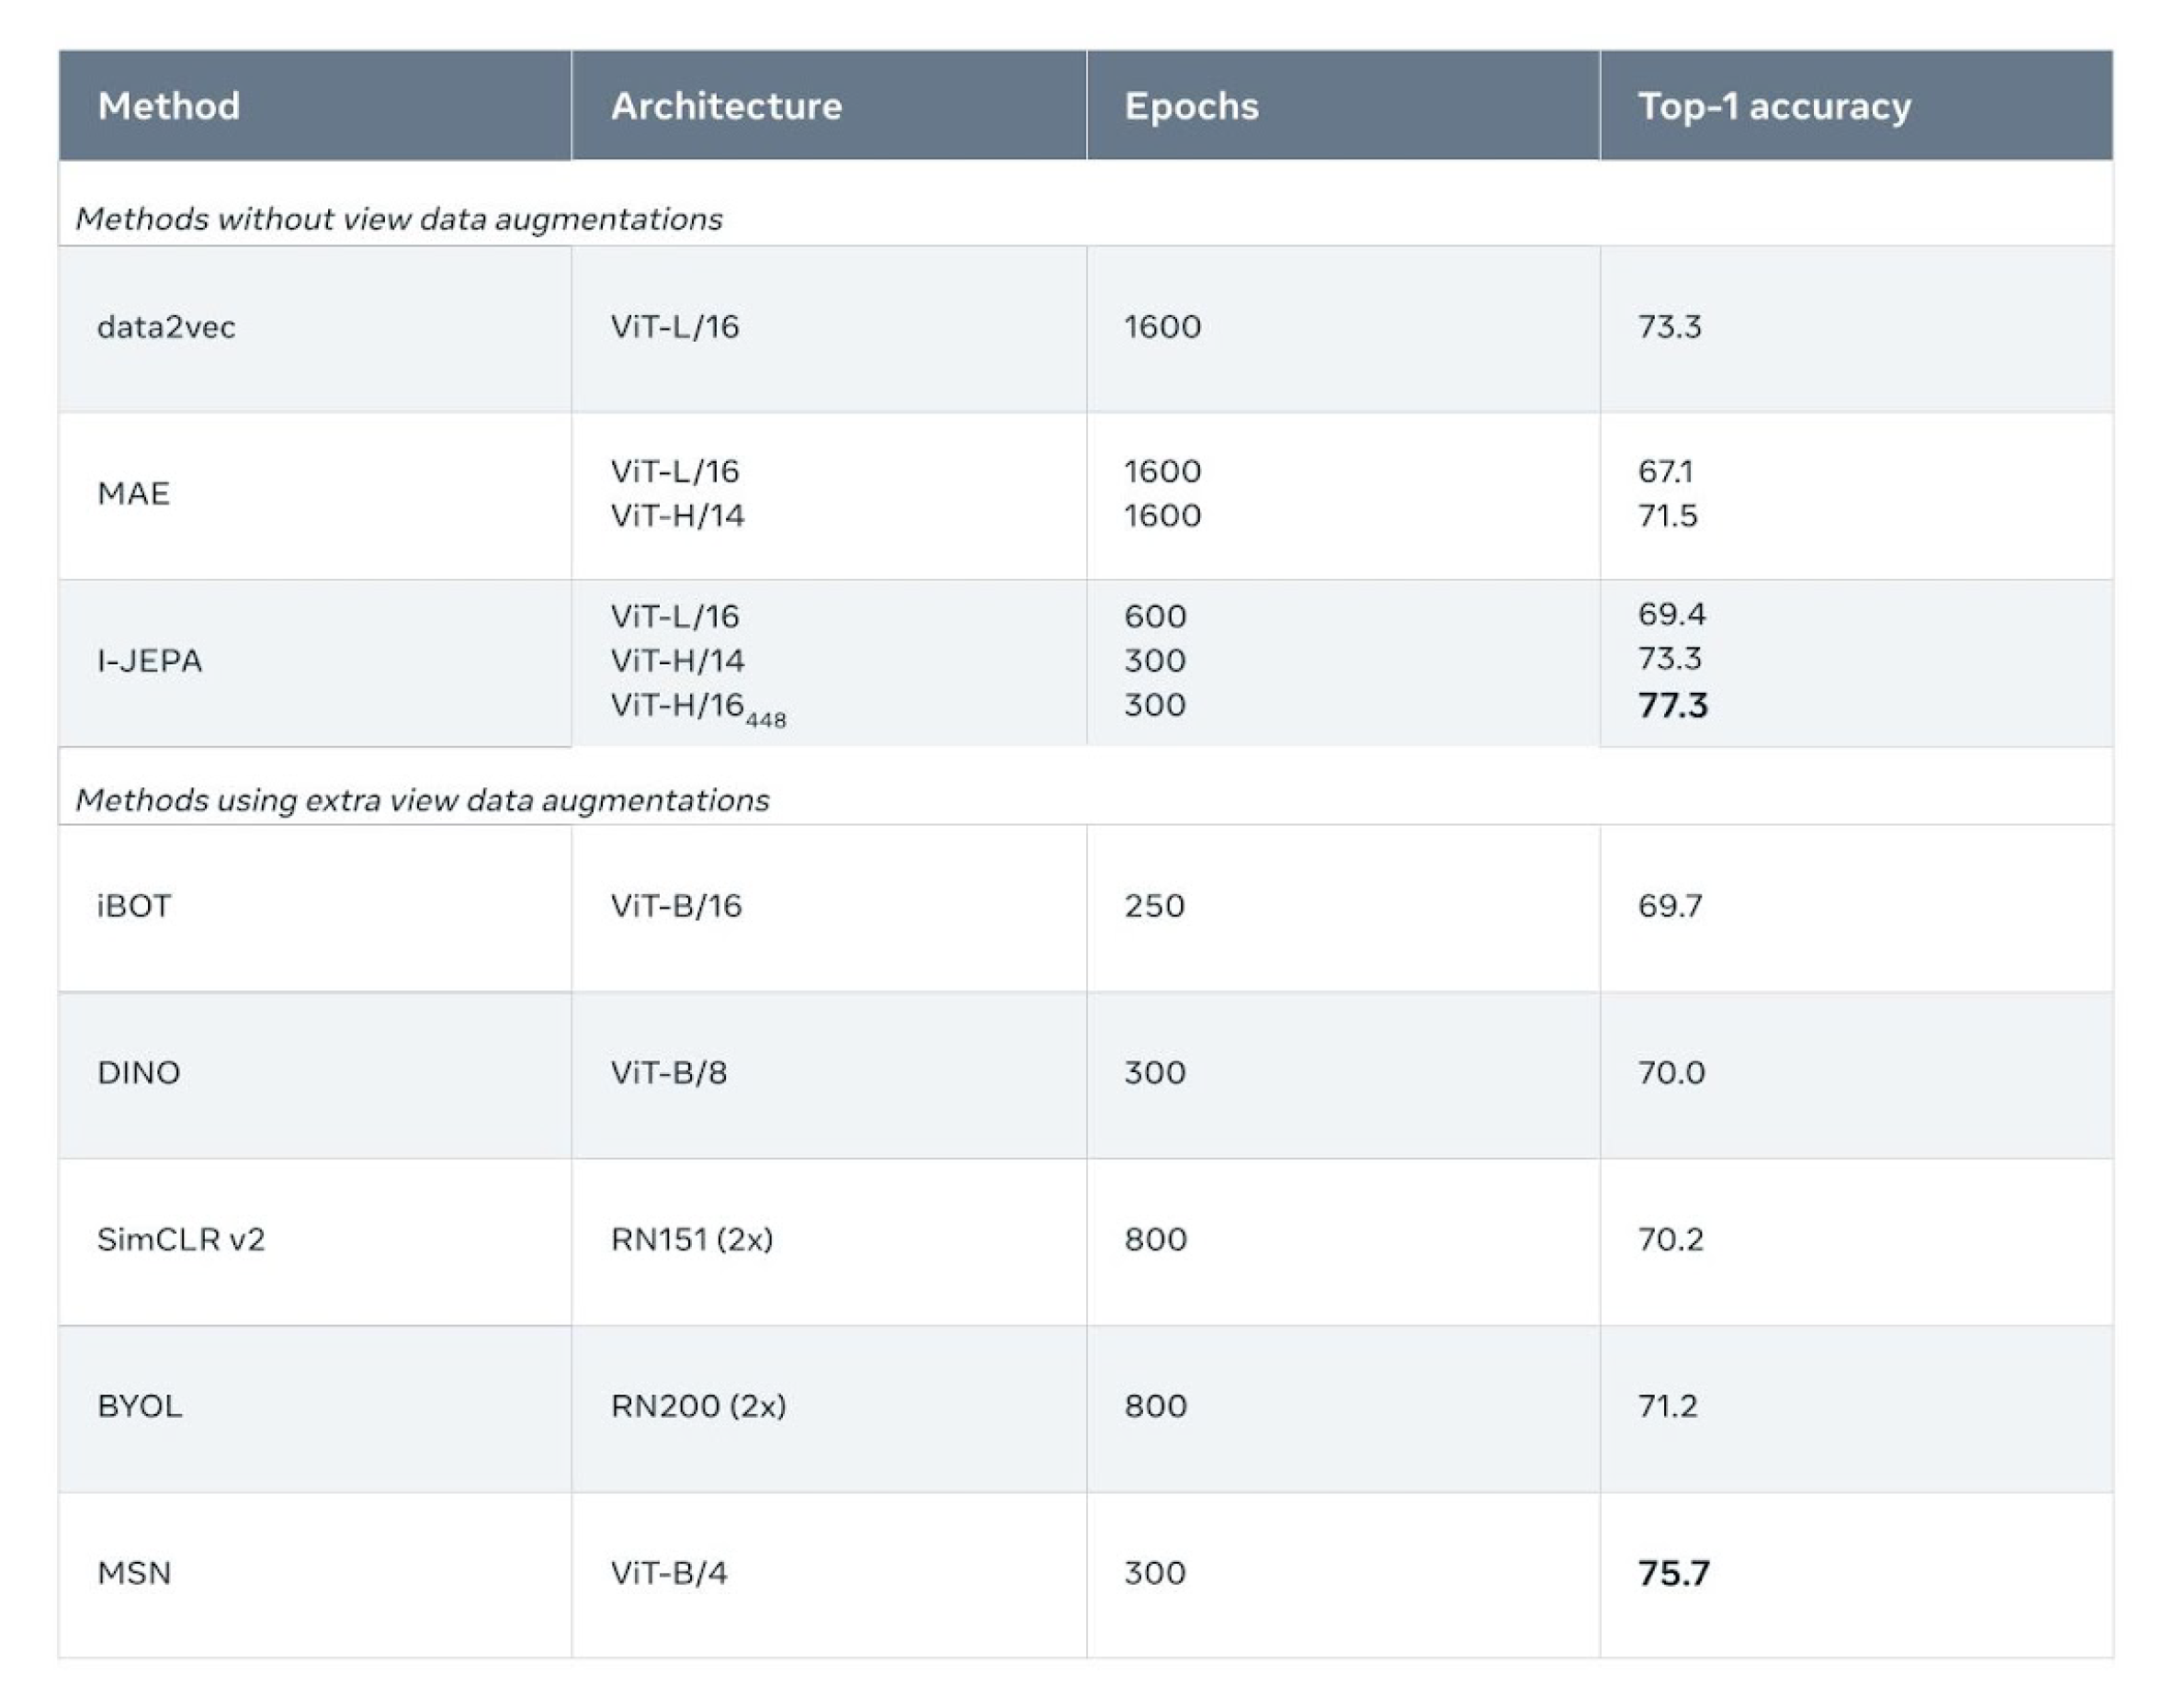
\includegraphics[width=0.8\textwidth, height=0.8\textheight, keepaspectratio]{assets/New-Lecture_JEPA_models/ijepa_blog_imagenet_linear_table.png}\\[0.35em]
  {\scriptsize Low Shot Classification Accuracy: Semi-supervised evaluation on ImageNet-1k with 1\% of the labels (approximately 12 labeled images per class).}
\end{frame}

% --- I-JEPA: Results and Applications ---
\begin{frame}{I-JEPA: Results and Applications}
  \begin{itemize}
    \item Strong \textbf{off-the-shelf} representations: linear probe, semi-supervised, and competitive low-shot settings without extensive task-specific fine-tuning of the backbone.
    \item Transfers to classification, detection, segmentation-style use cases; blog and paper emphasize \textbf{broader task mix} including some low-level vision tasks.
    \item Open direction: extend JEPAs to \textbf{richer modalities} (video, audio, text conditioning) for longer-horizon \textbf{world models}.
  \end{itemize}
\end{frame}

% --- Comparing SSL Architectures ---
% \begin{frame}{SSL Architectures: MAE vs. JEPA}
%   \centering
%   \includegraphics[width=0.9\textwidth]{assets/New-Lecture_JEPA_models/mae_vs_ijepa.png}
%   \begin{itemize}
%     \item \textbf{MAE:} Predicts pixels for masked regions, high reconstruction overhead.
%     \item \textbf{JEPA:} Predicts feature embeddings, abstracting visual content.
%     \item JEPA encourages more semantically meaningful representations.
%   \end{itemize}
% \end{frame}

